% \setlength{\tabcolsep}{1pt}
\begin{figure}[h]
    \small
    \centering
    \begin{tabular}{ccc}
      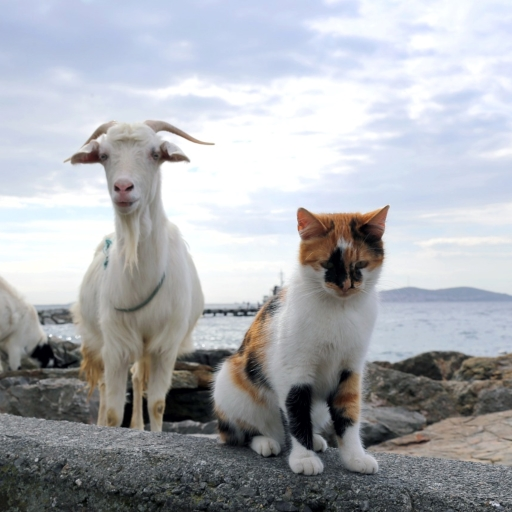
\includegraphics[width=1.8cm, height=1.8cm]{fig/cross_map_images/cross_image} & 
\includegraphics[width=1.8cm, height=1.8cm]{fig/cross_map_images/cat_map} & 
\includegraphics[width=1.8cm, height=1.8cm]{fig/cross_map_images/goat_map} \\
      Input & \textit{``cat"} & \textit{``goat"} \\
    %   \multicolumn{3}{c}{``\textit{a \textcolor{BrickRed}{\st{man}} \textcolor{RoyalBlue}{\textbf{woman}} smiling}"} \\
    %   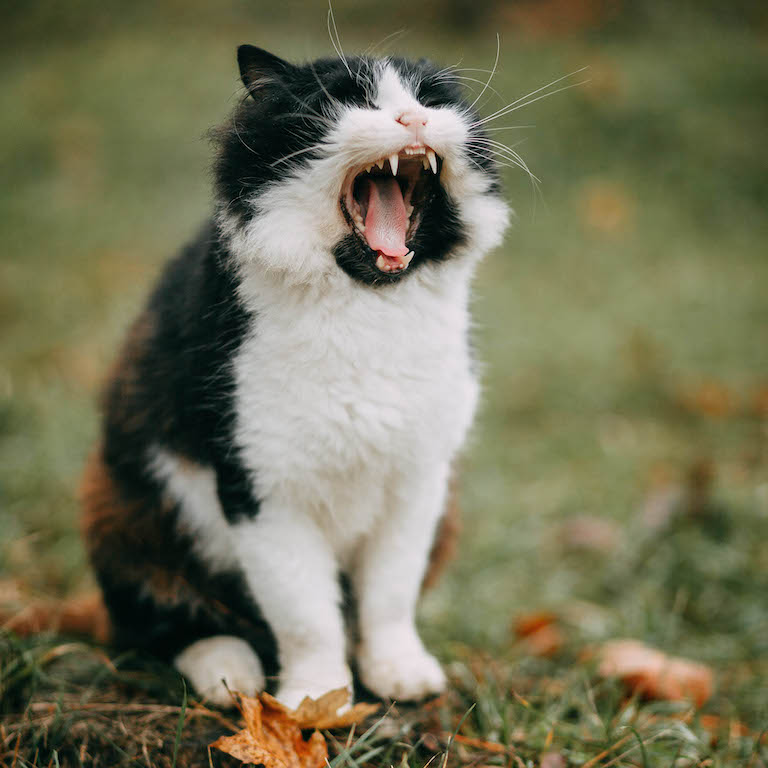
\includegraphics[width=2.2cm, height=2.2cm]{fig/teaser/teaser_2_in.jpg} & $\rightarrow$ & 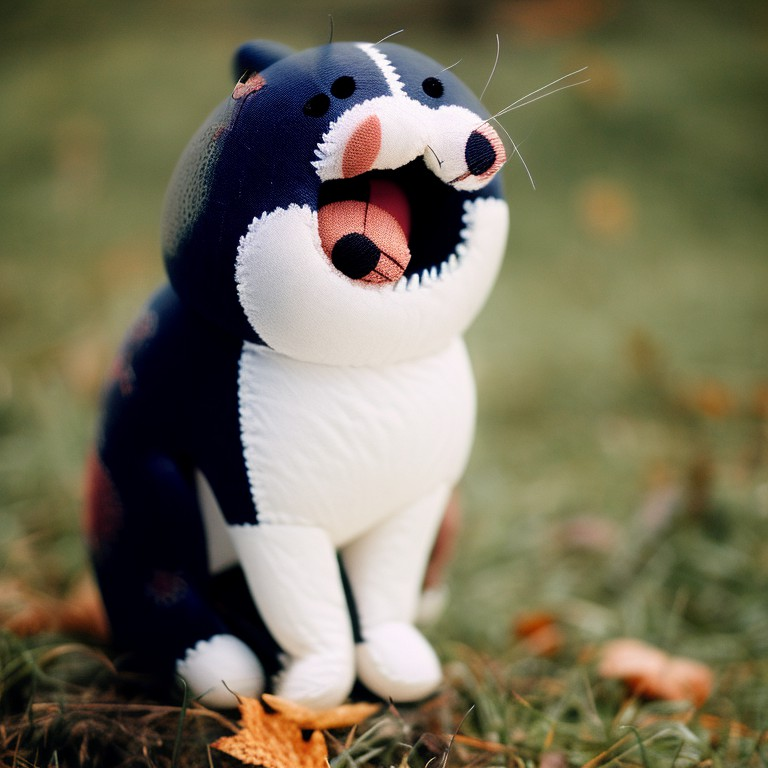
\includegraphics[width=2.2cm, height=2.2cm]{fig/teaser/teaser_2_out} \\
    %   \multicolumn{3}{c}{``\textit{a \textcolor{RoyalBlue}{\textbf{plush toy}} cat yawning }"} \\
      
    \end{tabular}
    \caption{Averaged $16 \times 16$ cross-attention maps corresponding to ``\textit{cat}" and ``\textit{goat}" for the input ``\textit{A cat and a goat}."}
    \label{fig:crossatt_map}
  \end{figure}

%   \begin{figure}
%     \includegraphics[width=0.99\linewidth]{fig/03_bird_and_bear.pdf}
%     \caption{Averaged cross-attention maps for the sentence "a furry bear watching a bird". The cross-attention maps corresponding to \textit{bird} and \textit{bear} are also shown across different timesteps. Figure taken from \cite{hertz2023prompt}. \guille{This is 100\% stolen from prompt-to-prompt but I believe it's really important for understanding what cross-attention maps are and what do they encode. How critital is that we make our own?}}
%     \label{fig:crossattn_viz}
%   \end{figure}
  